\documentclass[withoutpreface,bwprint]{cumcmthesis} %去掉封面与编号页
\usepackage[framemethod=TikZ]{mdframed}
\usepackage{url}   % 网页链接
\usepackage{subcaption} % 子标题、
\usepackage{graphicx}
\title{“信息引航者”——基于MGCA的信息推荐系统}
\usepackage{listings}
\lstset{language=Matlab}
\usepackage{pythonhighlight}
\usepackage{setspace}
\begin{document}
	
	\maketitle\thispagestyle{empty}
	\begin{abstract}
		随着互联网上信息的越来越多,想要在海量信息中获取我们感兴趣或有需求的信息愈加困难。推荐系统的出现正是为了解决这种\textbf{“信息过载”}的问题。推荐系统已在互联网中得到了广泛的应用,并给应用它的企业带来了\textbf{丰厚的利润}。有关推荐系统的研究具有十分深远的意义与巨大的实用价值,我们的项目\textbf{《 “ 信息引航者”——基于MGCA的信息推荐系统》 }就是为了解决“信息过载”问题,响应国家发展和改革委员会“新基建”号召,创造巨大经济价值而设计的一款推荐系统,并在此基础上进行了商业构想,制定了完整的商业计划。\par
		技术路线上,我们设计了一种\textbf{考虑多种粒度信息的候选感知推荐算法},并在微软发布的MIND数据集上进行新闻推荐任务,通过\textbf{知识图谱、图神经网络、Transformer、Fastformer}等基础模型组成\textbf{MGCA( Multi-grained Candidate-aware)模型},聚合不同粒度的候选感知信息与候选新闻匹配推荐用户兴趣咨询信息,在微软的MIND数据集Small版本新闻推荐任务成为\textbf{SOTA模型},暂时为该数据集上新闻推荐任务AUC、MRR、nDCG等指标\textbf{最高的模型},比2022年清华大学Tao Qi等人提出的SOTA模型KIM的AUC、MRR、nDCG@5,nDCG@10指标分别高\textbf{1.00、1.33、0.63、0.96}个百分点。\par
		商业计划上,我们制定了完整的创新商业构建。产品营销定位\textbf{全国由于算法、算力壁垒急需但难求个性化推荐系统的中、小企业},致力于助力中、小企业拥有自己的个性化推荐系统,促进推荐系统的广告、增值服务、电商、节省成本变现。盈利方式聚焦B端企业,提供\textbf{低耦合工业界解决方案或完整软件系统},适应不同类型企业的不同需求。财务管理单设财务部进行,其中软件成本计算采取Barry Boehm提出的\textbf{COCOMO模型}。市场竞争分析按照\textbf{SWOT模型}进行分析,充分考虑团队优势劣势。营销方式上,根据Raymond Vemon教授的\textbf{产品生命周期理论},按照团队发展的不同阶段采取不同的营销模式。营销策略上不同于传统的“7P+4C”策略,我们采取\textbf{“六位一体”的扁平化多层化营销策略}。\par
		工程落地上,我们在\textbf{Python3.6和Tensorflow1.15}框架的环境下进行算法的研发设计与实验研究,在\textbf{JAVA jdk1.8}的环境下,前端采取\textbf{Vue3、Bootstrap}框架,后端采取\textbf{SpringBoot}框架进行软件开发。在完整软件开发的流程中,采取\textbf{原型软件生命周期模型}组织开发,不断适应复杂多变的需求,提高B端企业客户体验,为了规避原型模型难以规划和管理的弊端,\textbf{定期核验开发进展},进行\textbf{兼容性测试与稳定性测试},确保项目正常运行。\par
		\textbf	{关键字: MGCA( Multi-grained Candidate-aware)模型\quad  COCOMO模型\quad  SWOT\quad  “六位一体”扁平多层化营销策略\quad   Tensorflow\quad SpringBoot\quad  原型软件生命周期模型\quad	}
	\end{abstract}
	\setcounter{page}{1}
	\tableofcontents
	\newpage
	\section{引言}
	\subsection{研究背景及意义}
	\subsubsection{ 信息过载问题的解决迫在眉睫} 
	互联网高速发展,信息呈爆炸式增长,用户逐渐由信息匮乏时代迈入了信息过载时代——过量信息反而使得用户无法找到自己需要的信息。信息过载问题会产生一系列问题,比如用户体验变差、用户数量骤减、用户粘性降低等。
	信息爆炸的今天,个性化新闻推荐技术已经变成了许多新闻网站和App的关键技术。新闻的数据来源众多,可能一分钟就有成千上万条新的数据产生,在数据量激增的情况下,需要付出更多的人力成本,并且人工处理速度慢,效率十分低下。一套个性化新闻推荐系统刚好可以应用于有效缓解这种信息过载问题。如图1是新闻推荐系统通过个性化推荐实现精准化投放信息的流程示意。
	\begin{figure}[H]
		\centering
		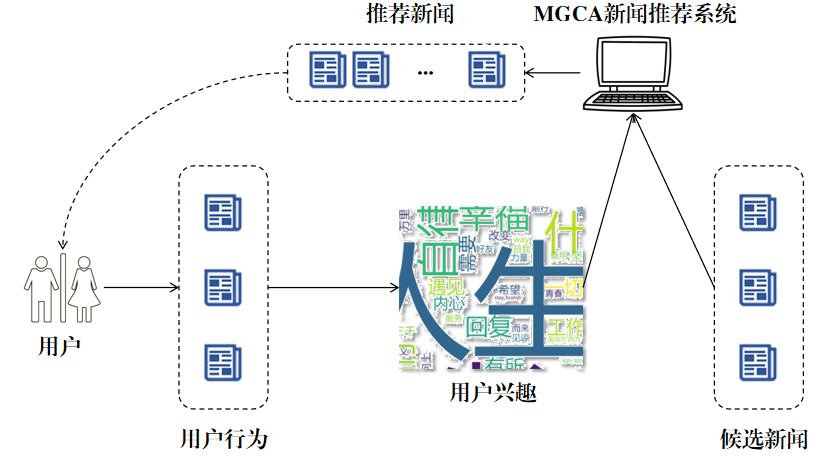
\includegraphics[width=0.95\textwidth]{2}
		\caption{个性化新闻推荐系统实现精准化投放信息}
		\label{fig:circuit-diagcam}
	\end{figure}
	\subsubsection{ 互联网与推荐系统的融合带来巨大的经济价值}
	目前互联网变现的主要方式均可以与推荐系统融合起来,创造巨大的经济价值,如图2展示了推荐系统与互联网融合时创造价值的几种常见途径:
	\begin{figure}[H]
		\centering
		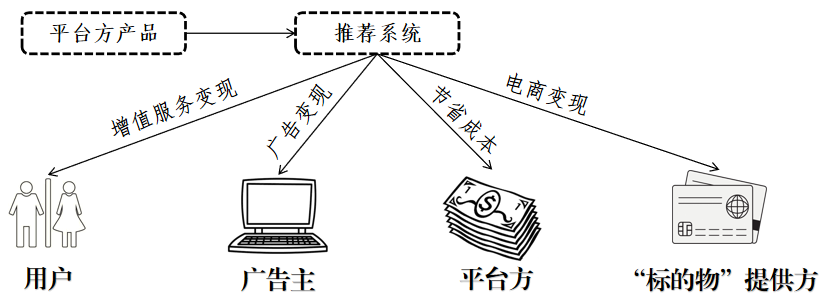
\includegraphics[width=0.95\textwidth]{1}
		\caption{推荐系统与互联网融合体现的经济价值}
		\label{fig:circuit-diagcam}
	\end{figure}
	$\bigstar$\textbf{广告变现:}用户方产品在互联网上投放广告,通过提高广告曝光以及用户点击广告获取权益。通过推荐系统的应用,可以在新闻APP中实现广告精准投放。广告业务偏轻公司一般都会选择流量外包方式做广告变现,\textbf{通过推荐系统提高广告精准投放率与用户点击率即是一种非常好的方式。}\par
	$\bigstar$\textbf{增值服务变现:}增值服务主要是指基本服务以外的特色服务,如新闻平台常见的会员制。推荐系统通过精准把握用户兴趣,引导用户购买会员增值服务产品。推荐系统的个性化推荐服务不仅可以更加深层次的挖掘用户需求,还可以使更多相对冷门但优质的内容得到曝光与展示。在 2004 年,一位杂志主编在形容亚马逊和 Netflix 的商业模式时首次提出“长尾”概念,指代需求和销量不高的产品在市场中所占比例与主流产品相当甚至更高。当传统的二八定律无法再创造更多利润时,商家开始关注“长尾”潜在的商业价值,即专注于小众群体的个性化偏好。\textbf{推荐算法在实现企业从二八定律向“长尾效应”转变方面发挥着重要作用。}以往市场只关注大众需求,而通过推荐系统,个性化需求也可以得到满足,提高了用户的满意程度和消费质量,实现了双赢。\par
	$\bigstar$\textbf{节省成本变现:}在推荐算法还不作为推荐系统的重要组成部分之前,推荐这项工作的大部分还是由人工完成的,根据一些专业人士的建议和想法,来向用户推荐产品及服务。推荐系统对平台方的贡献不仅在于直接的商业价值或是促进用户粘性、用户数量增长等,还可以\textbf{用更少的成本实现最大程度的个性化新闻推荐,提高内容的分发效率。}\par
	$\bigstar$\textbf{电商变现:}无论是传统意义的实体电商产品,还是网络小说、网络课程等虚拟电商产品,都可以通过提高分发商品效率,精准化投放促进商品售卖而提高商家分成,吸引商家入驻。总的来说,\textbf{在电商变现方面,推荐系统可以做到促进“标的物”提供方的生态逐步健全繁荣,获取更多经济效益。}\par
	\subsubsection{ 响应国家发展和改革委员会“新基建”号召}
	国家发改委于2020年4月首次明确了新型基础设施的范围包括以人工智能、云计算、区块链等为代表的新技术基础设施,新型基础设施建设对于打造经济新动能、重塑供应新链条、促进惠民新模式有重大意义,是当前稳经济、促增长的核心支撑。人工智能、云计算、物联网等现代信息科技依托新型基础设施建设得到了高速发展。\par
	特别是处于疫情后时代,线下娱乐受到重创,线上娱乐成为青年群体最重要的娱乐方式之一。在当前的时代背景下,推荐系统的研究有助于\textbf{促进青年群体的幸福感,扩大新型基础设施建设的有效投资,有效对冲经济下行压力,有力支撑经济社会高质量恢复与持续发展。}
	\subsection{相关研究现状}
	推荐系统是学术界和工业界研究的热门话题。学术界侧重理论层面的分析和模型性能的提升,而工业界更侧重实践层面的发展以及用户体验的提升以及推荐系统的应用前景。下面从这两方面分别介绍。
	\subsubsection{ 推荐系统在工业界的应用与发展前景}
	在移动互联网快速发展、智能手机普及以及信息产生爆炸增长的背景下,高效获取对个人有价值的信息变得愈发重要。推荐系统作为一种高效的信息过滤工具,在用户精准高效获取信息方面起到了重要作用。它不仅解决了用户需求不明确时的信息获取问题,也在内容分发、用户体验和商业变现方面发挥着关键作用。推荐系统已经成为toC互联网产品的标配技术,并给应用它的企业带来了丰厚的利润。据报道,推荐系统给亚马逊带来了35\%的销售收入,给Netflix带来了高达75\%的消费,并且Youtube主页上60\%的浏览来自推荐服务。如下表1所示,常见的推荐系统以及推荐内容与使用的特征表,展示了国内应用了推荐系统的常见应用。\par
	\begin{table}[H]
		\centering
		\caption{不同推荐场景下的推荐内容和特征}
		\begin{tabular}{|m{2cm}|m{4cm}|m{4cm}|m{4cm}|}
			\hline
			推荐场景 & 推荐产品 & 推荐项 & 推荐使用的特征 \\
			\hline
			资讯推荐 & 今日头条、百度新闻、腾讯新闻、知乎 & 新闻标题、内容、主题 & 用户行为、用户画像、年龄、性别、教育背景 \\
			\hline
			快资讯 & 抖音、快手、西瓜视频、YouTube & 视频内容、音频、类型 & 热度、标题和描述、用户行为 \\
			\hline
			腾讯视频 & 爱奇艺、优酷、HBO、Netflix & QQ音乐、网易云音乐 & 音频类型、演唱者、作曲者等 \\
			\hline
			电商推荐 & 淘宝、京东、亚马逊、拼多多 & 商品 & 商品标题、描述、图片、类别、流行度 \\
			\hline
		\end{tabular}
	\end{table}
	推荐系统的发展与大环境和技术进步密不可分,接下来我们从三个层面分析推荐系统发展的前景:\par
	$\bigstar$\textbf{政策层面:}在当前“智能化”的时代背景下,国家空前把人工智能提升到了战略的高度,政策的大力支持、媒体的大肆宣扬以及样板示范作用,让个性化新闻推荐的产品与业务受到了更多投资人、专家的重视,这不仅极大推动了新闻推荐系统的发展,也有利于推荐系统在更多的业务场景下落地。\par
	$\bigstar$\textbf{教育层面:}国内从2016年起步开始开设数据科学与大数据技术、智能科学与技术等人工智能相关专业,推荐系统作为大数据和人工智能领域业务价值最大之一的领域,极大的受益于大数据与人工智能相关学科人才的增长,这为助力推荐系统进一步发展提供了基础。\par
	$\bigstar$\textbf{科技层面:}构建一套灵活实时、准确度高、稳定高效的新闻推荐系统是非常困难的,它不仅涉及到业务场景,还与产品交互、工程应用密不可分,几乎只有中、大规模的公司才会构建一套推荐算法业务体系,但受益于云计算基础设施的逐步健全,创业公司可以利用云平台提供的SAAS服务搭建自己的推荐系统模块,降低了推荐系统的使用门槛,促进了推荐系统更加广泛的应用。\par
	\subsubsection{ 推荐系统在学术界的研究现状}
	根据用户日志的数据的输入形式和推荐算法的设计机制,推荐系统在学术界的发展主要包含以下三个阶段:基于协同过滤的推荐、基于内容的推荐以及混合推荐。\par
	$\bullet$\textbf{基于协同过滤的推荐:}协同过滤推荐算法是诞生最早且比较著名的推荐算法,这种算法主要考虑了用户与与用户之间的相似度,在所有用户群体中找到与用户具有相似兴趣、相似偏好的的用户感兴趣的产品或服务推荐给用户。例如下图3中的情景,小林喜欢《间谍过家家》和《干物妹小埋》这类喜剧动漫片,小浩也喜欢看喜剧动漫,如《间谍过家家》、《干物妹小埋》和《工作细胞》等。基于相似喜好,在协同过滤算法中会将小林未看过但小浩喜欢的动漫《工作细胞》推荐给小林。\par
	\begin{figure}[H]
		\centering
		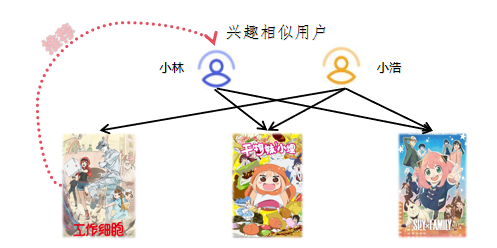
\includegraphics[width=0.65\textwidth]{3}
		\caption{协同过滤推荐示例}
		\label{fig:circuit-diagcam}
	\end{figure}
	目前学术界已提出多种协同过滤的推荐算法,包括传统的矩阵分解方法和结合深度学习技术的新型方法。传统方法存在冷启动和数据稀疏等问题,而深度学习结合的方法如Autoencoders、CDAE和DMF能更好地解决这些问题,通过学习用户和项的潜在因子来提高推荐性能。尽管协同过滤在工业界得到广泛应用,但仍面临冷启动等挑战,需要进一步研究完善。\par
	$\bullet$\textbf{基于内容的推荐:}这种算法不同于协同过滤算法,根据用户的交互记录为用户提供个性化推荐结果,基于内容的推荐算法的基本原理是根据用户和项的属性特征以及用户的历史行为,获得用户的兴趣偏好,为用户推荐跟他的兴趣偏好相匹配的项。例如小琰经常浏览与各地旅游攻略相关的资讯,基于内容的推荐算法则可能推荐近期爆火的旅游地相关新闻。\par
	基于内容的推荐方法早期采用统计策略,如TF-IDF和余弦相似度,存在内容相同但物品不同的问题。后续方法利用机器学习技术如决策树、最近邻居和神经网络解决这一问题,比如DeepWide和DeepFM。目前主流的基于深度神经网络的推荐算法使用CNN、RNN、注意力网络或记忆网络从用户历史交互序列中提取特征,例如DeepJoNN、ATEM和MANN。为克服错误关系假设,一些方法利用神经网络挖掘用户的长期兴趣和短期兴趣,融合长短期兴趣做个性化推荐,这称为以会话为主的推荐方法。\par
	$\bullet$\textbf{混合推荐:}混合推荐算法进一步提升了推荐系统的性能,融合了知识图谱的信息,增加了推荐系统内部算法的可解释性。利用知识表示学习技术将丰富语义信息融入推荐过程,使结果更准确满足用户需求。混合推荐方法建立用户知识图谱,利用路径推理、强化学习和图神经网络技术将购买关系建模为知识图谱的补全任务,从中学习用户和项的表示并预测匹配概率,即向用户推荐该项的概率。比如较为经典的 KPRN 方法使用循环神经网络挖掘用户与物品之间的图谱路径,利用知识图谱的路径推理技术建模用户与候选推荐项的可解释性推荐。这一前沿技术解决了推荐算法黑盒问题,提高了推荐结果的可解释性,是未来推荐系统的重要研究方向。\par
	表 2 列举了上述三类方法的经典模型、各模型使用的核心技术以及评测指标等。
	\begin{table}[H]
	\centering
	\caption{三类方法的核心技术对比}
	\begin{tabular}{|m{2cm}|m{4cm}|m{4cm}|m{4cm}|}
		\hline
		推荐场景 & 方法举例 & 核心技术 & 评价指标 \\
		\hline
		协同过滤推荐方法 & Autoencoders、CADE、DMF、CKE & 矩阵分解、张量分解、神经网络 & accuracy、MRR、ndcg@k \\
		\hline
		基于文本内容推荐 & TransRec、DeepCoNN、JRL、DKN、DAN & 卷积神经网络、循环神经网络、注意力机制 & accuracy、MRR、ndcg@k \\
		\hline
		混合推荐方法 & KPRN、RippleNet、KGCN、VGAE、PGPR & 强化学习、图卷积神经网络、深度神经网络、注意力神经网络 & accuracy、MRR、ndcg@k \\
		\hline
	\end{tabular}
	\end{table}
	\subsection{项目架构总览}
	\subsubsection{ 项目整体框架}
	本项目的整体框架主要包含营销策略、模型框架、工程落地三个阶段,结合了实际应用和技术发展趋势,就创新业务做商业计划分析和原型搭建,实现了IT与业务的相对齐。\par
	\begin{figure}[H]
		%\centering
		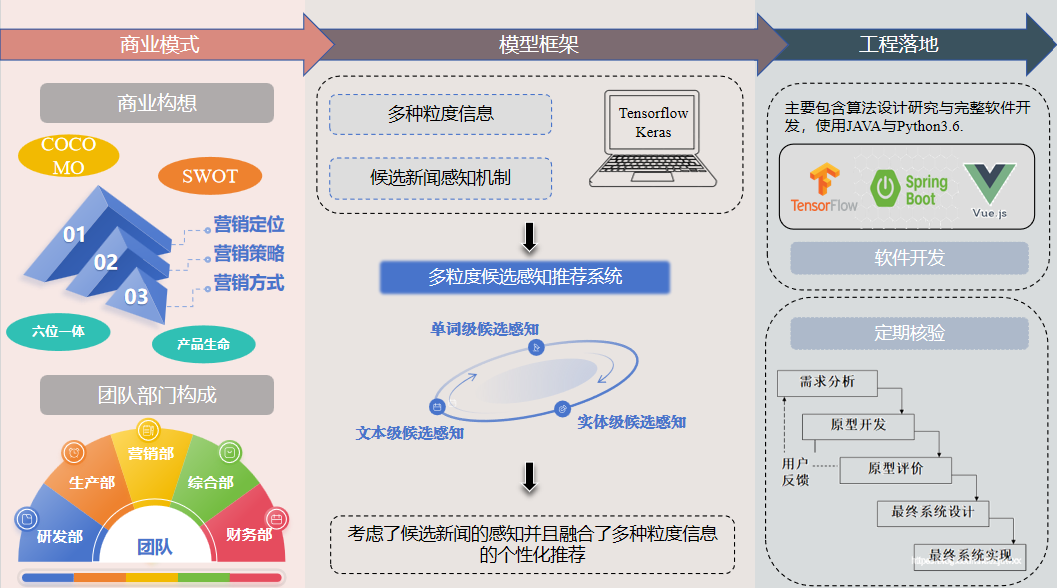
\includegraphics[width=1.0\textwidth]{框架}
		\caption{项目框架图}
		\label{fig:circuit-diagcam}
	\end{figure}
		$\bigstar$\textbf{模型框架:}基于之前的研究,我们提出了一种融合多种粒度信息的候选感知推荐系统,并在微软的公开数据集MIND数据集上进行新闻推荐任务上得到了截止目前AUC、MRR、nDCG@5,nDCG@10等指标最高的模型,在transformer头数、fastformer头数、学习率、优化器等参数确定情况下,比2022年清华大学Tao Qi等人在Personalized News Recommendation with Knowledge-aware Interactive Matching中提出的SOTA模型KIM的AUC、MRR、nDCG@5,nDCG@10指标分别高\textbf{1.00、1.33、0.63、0.96}个百分点,是该数据集的Small版本当前国内AUC、MRR、nDCG@5,nDCG@10指标最高的模型。\par
		模型的算法框架主要包含两个部分:多粒度用户点击新闻编码器、候选新闻编码器。多粒度用户点击新闻编码器主要包含单词级、新闻级、实体级三种粒度的信息,可以充分挖掘用户点击的信息在不同粒度信息的潜在内容,更加细致的挖掘用户兴趣,其中实体级粒度编码器与候选新闻编码器中的实体信息是与用户点击新闻通过知识编码器交互式学习得到。在候选新闻编码器中,候选新闻通过新闻编码器得到的信息与知识编码器中得到的信息聚合后再次通过Transoformer、Fastformer聚合到用户点击新闻中,最终聚合三个粒度的信息与候选新闻编码器得到了候选新闻信息进行匹配得到匹配分数,进行个性化新闻推荐。这样的推荐不仅感知了候选新闻与用户历史点击新闻的关联信息,还考虑了不同粒度信息中不同的潜在推荐价值,相比以往模型具有显著优越性。如下图5所示,算法框架的整体结构图。\par
		\begin{figure}[H]
			%\centering
				\includegraphics[width=1.0\textwidth]{MGCA}
			\caption{算法架构图}
			\label{fig:circuit-diagcam}
		\end{figure}
	    $\bigstar$\textbf{商业计划:}本产品营销定位全国由于算法、算力壁垒急需但难求个性化推荐系统的中、小企业,致力于助力中、小企业拥有自己的个性化推荐系统,促进推荐系统的多元化变现,提高广告的转化率与曝光、促进“标的物”提供商家的生态繁荣、促进“标的物”售卖。ToB,指公司的产品或服务所面向的用户是企业,围绕企业的生产、管理、运营、决策等环节制定相应的产品服务,团队盈利方式\textbf{聚焦toB端},主要包含\textbf{提供整套低耦合工业界解决方案和成熟的整套解决方案}。低耦合工业界解决方案通过提供近零耦合的代码段供企业直接聚合到自己推荐系统中创造价值。同时在我们的商业计划构想中,团队包含专业的软件开发人员,可以直接为不具备软件开发能力的企业直接提供成熟的整套软件,满足企业的个性化需求,并且将我们的推荐系统嵌入其中。团队会建立商业量化指标体系,保证推荐系统真正的落地业务。\par
	    团队成立初,共包含研发部、生产部、营销部、综合部、财务部等部门。团队成立初产品类型有限,但软件开发需求复杂多变,团队成立生产部用于进行软件开发活动。设立财务部单独管理财务,其中,软件开发的成本估算采用Barry Boehm在1981年提出的\textbf{COCOMO模型}计算,这是一种基于代码行的回归模型,考虑了软件项目开发过程中的大小、工作量、成本、时间、质量。
	    在市场竞争分析中,我们使用\textbf{SWOT模型}进行分析( Strengths,Weakness,Opportunesses,Treats),充分考虑了团队的优势、劣势、机会和威胁风险之间的关系。
	    在营销模式中,根据Raymond Vemon教授的产品生命周期理论,我们按照团队发展的三个阶段( 前期、中期、后期)制定了不同的营销模式。不同于传统的“7P+4C”营销策略,我们采取\textbf{“六位一体”式的扁平化多层化式营销方式}。\par
	    $\bigstar$\textbf{工程落地:}在算法的研发和设计阶段在\textbf{Python3.6的Tensorflow框架}下进行,使用VSCode、Pycharm等工具进行编码实现与实验研究。在完整的软件方案开发过程中,我们主要使用JAVA在jdk1.8环境下进行,前端框架主要采取\textbf{Vue3,bootstrap},后端框架主要采取\textbf{SpringBoot},开发平台选用IDEA。在软件开发的周期中,为了应对模糊不清、复杂多变的需求,我们采取\textbf{原型模型}的思想组织软件开发人员进行开发,在开发过程中不断适应需求、增进对需求的理解,对于B端企业客户也是学习使用软件的过程,便于确定系统的性能、服务的质量、设计的可行性,同时,为了规避原型软件周期模型难以规划和管理的缺点,团队将组织定期\textbf{核验开发进展},确保开发顺利进行。在软件开发过程中,我们严格按照软件开发流程进行\textbf{数据库E-R图设计、UML设计},并在每次的核验中进行兼容性与稳定性测试,确保项目正常运行。\par
	\subsubsection{ 项目优势与创新性}
	$\bigstar$\textbf{算法考虑了多种粒度信息的候选新闻感知,适应用户不同粒度的行为信息:}以往的模型有些虽然考虑了用户点击新闻与候选新闻的关联信息,但它们仅仅只是将候选新闻与用户的兴趣进行建模,没有将其融合到多种粒度的信息中考虑,我们的模型考虑多种粒度信息的候选新闻感知,在微软的MIND数据集Small版本上成为当前任务的\textbf{SOTA模型},暂时在AUC、MRR、nDCG等指标\textbf{领先国内},下面的例子可以很好的具象化我们模型的优越性:如图6所示,第一个点击的新闻包含了“拼多多”、“买家秀”,这些词与第一个候选新闻的“拼多多”有关。第二个点击新闻也与第一个候选新闻有单词级的关联,因为它们都包含同一个单词“拼多多”。基于单词级的相关性可以推断用户可能对第一个候选新闻感兴趣。使用知识图谱进行点击新闻和候选新闻之间的实体匹配,有助于更好地理解用户对候选新闻的兴趣。例如,第三个点击新闻中的实体“《 黑铁的鱼影》” 与第二个候选新闻中的实体“《 名侦探柯南》” 具有固有的相关性。《黑铁的鱼影》是《名侦探柯南》 的剧场版影视,通过知识图谱根据实体级匹配可以推断出用户可能对第二个候选新闻感兴趣。因此,利用不同粒度信息之间的相关性有利于兴趣匹配。\par
	\begin{figure}[H]
		\centering
		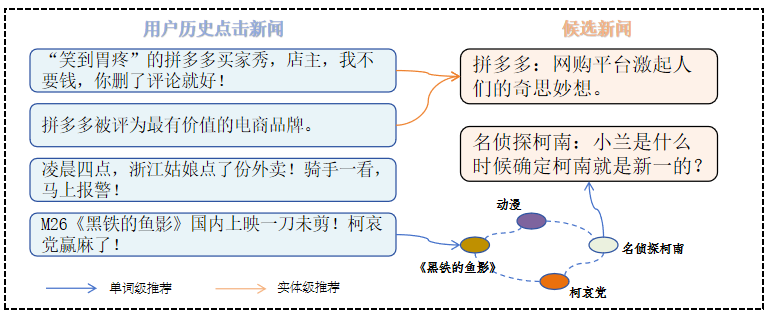
\includegraphics[width=0.9\textwidth]{sample}
		\caption{体现不同粒度信息对于新闻推荐重要性的一个例子}
		\label{fig:circuit-diagcam}
	\end{figure}
	$\bigstar$\textbf{商业计划完善,可以适应市场变化:}我们的市场定位非常清晰——聚焦B端企业。我们制定了完善的商业计划,包含了完整的团队构成、财务计算方法、市场竞争分析和营销策略方法。团队构成上研发部、生产部、营销部、综合部、财务部各司其责,完成算法改进、软件开发、宣传营销、协助协调。财务管理等各自要务,并且保持交流沟通。财务计算方法上创新性的采用了COCOMO模型计算软件开发成本,按照基础、中级、细致三个模型阶段分别计算,精确掌握开发成本,合理定价,适应市场变化。\par
	在营销策略中创新性的采取“六位一体”的扁平化多层化营销策略,如下图7,我们按照团队发展的前期、中期、后期三个阶段,分别制定了不同的营销模式,主要包含前期营销模式( 互联网云平台营销、线下开放式营销、服务体验与客户开发式营销)、中期营销模式( 中间商代理营销、专家营销)和后期营销模式( “ 一对一”互动制定化营销、品牌营销)。在互联网时代,三个时期的营销模式中我们都与互联网紧密结合,试图碰撞出更大的火花。\par
	\begin{figure}[H]
		%\centering
		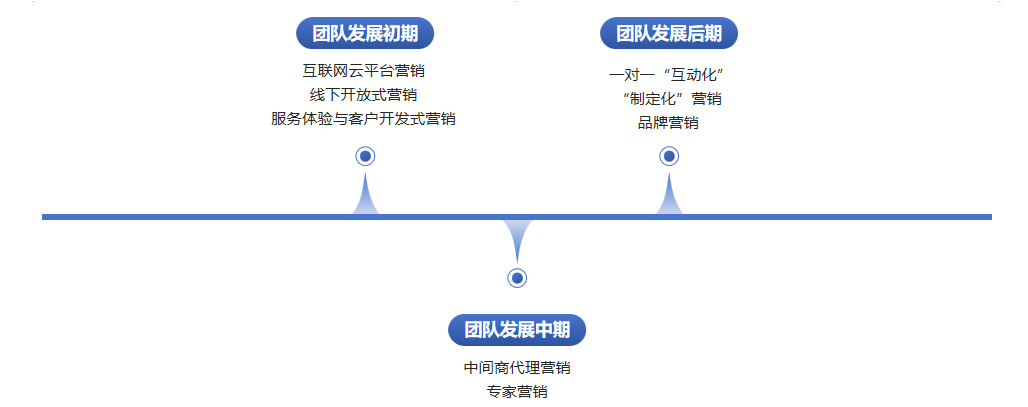
\includegraphics[width=0.95\textwidth]{营销发展}
		\caption{团队发展的不同时期采取不同的营销模式}
		\label{fig:circuit-diagcam}
	\end{figure}
	$\bigstar$\textbf{软件开发流程专业,适应B端企业的个性化需求:}团队人员具备专业的软件开发能力,为B端企业提供两种方案——低耦合工业界解决方案和成熟软件系统,以适应不同企业的需求。在下文中我们给出了一个完整的软件项目落地示例,软件生命周期采取了原型化模型的思想,不断地具象化最终的完整软件,在此过程中方便B端企业客户不断适应软件的使用,并且及时修改,满足企业端客户的个性化需求。此外,我们通过定时核验的兼容性测试与稳定性测试规避了原型模型难以规划和管理的缺点。\par
	\newpage
	\section{模型技术路线及实现方案}
	\subsection{模型架构}
	给定用户$u$和候选新闻$n^c$,我们需要计算用户$u$对候选新闻$n^c$内容的兴趣度量相关性分数$z$。然后根据相关性分数对不同候选新闻进行排序并向用户$u$推荐。
	用户$u$与他/她点击的新闻集合$\{ c_1, c_2, \dots, c_m\} $相关,其中$c_i$表示第$i$次点击的新闻,$m$是点击新闻的数量。设$E$表示新闻$c$中的实体。
	我们假设新闻$c$通常会诱导$k$类文本信息(例如标题和实体)$T = \{ T_1, T_2,\dots, T_k\} $,其中$T_i$是新闻文本的第$i$类文本。文本序列$T_i$由多个令牌组成:$T_i = \{ t_{ i,1}  t_{ i,2}  ,\dots, t_{ i,l} \} $,其中$t_{ i,j} $是序列$T_i$中的第{ $j$} 个单词令牌,$l$是序列的最大长度。
	\subsubsection{ 候选新闻编码}
	\textbf{News Encoder.} 
	To differentiate between candidate news and user clicked news, we add the superscript “c” to the representation associated with candidate news.
	We first map each word $t^c_{ij}$ of the $i$-th genre of candidate news text $T_i^c$ into a $d_w$-dimensional vector $\mathbf{t}_{ij}^c \in \mathbb{R}^{d_w}$, where $d_w$ is embedding size dimension. Hence, the text $T_i^c$ can be represented as a feature map $\mathbf{T}_i^c = [\mathbf{t}_{i1}^c; \mathbf{t}_{i2}^c; \dots; \mathbf{t}_{il}^c]$, where $\mathbf{T}_i^c \in \mathbb{R}^{l \times d_w}$. 
	Transformer architecture is based on self-attention mechanisms, which allow the model to weigh the importance of different words in a sequence. It replaces recurrent neural networks (RNNs) traditionally used in sequence-to-sequence tasks and has shown superior performance in capturing intricate semantic and syntactic relationships among words. Thus, we adopt Transformer to model different genres of textual information. As Figure~\ref{newsencoder} shows, the contextualized word representations of the \textit{i}-th genre of textual information $\hat{\mathbf{T}}_i^c$ can be represented as follows:
	\begin{equation}\label{eta}
	\begin{split}
	\hat{\mathbf{t}} _{i1}^{c}, \hat{\mathbf{t}}_{i2}^{c}, \ldots, \hat{\mathbf{t}}_{il}^{c} =\mathrm{Trans} (\mathbf{t}^c_{i1},\mathbf{t}^c_{i2}, \ldots, \mathbf{t}^c_{il})\\
	\hat{\mathbf{T}}_i^c = [\hat{\mathbf{t}}_{i1}^{c}; \hat{\mathbf{t}}_{i2}^{c}; \ldots; \hat{\mathbf{t}}_{il}^{c}]
	\end{split}
	\end{equation}\label{eta}
	where $\hat{\mathbf{T}}^{c}_i \in \mathbb{R}^{l \times d_w}$, 
	The high-level feature vector of the $i$-th candidate news text $T_i^c$ is generated: 
	Soft Attention Mechanism.
	\begin{equation}
	\hat{\mathbf{t}^c_i} = softmax( \mathbf{W} \cdot \mathbf{(\hat{\mathbf{T}}^c_i})^{T} + \mathbf{b}) \cdot \mathbf{\hat{\mathbf{T}}^c_i}
	\end{equation}
	where $\hat{\mathbf{t}}^c_i \in \mathbb{R}^{d_w}$,$\mathbf{W}$ denotes trainable weight matrix and $\mathbf{b}$ denotes the bias term.
	The representations of all genres of news text are concatenated as the textual representation of the candidate news:
	\begin{equation}\label{eta}
	\mathbf{d}^c= \hat{\mathbf{t}}_1^c \oplus \hat{\mathbf{t}}_2^c \oplus \ldots \oplus \hat{\mathbf{t}}_k^c
	\end{equation}\label{eta}
	where $\mathbf{d}^c \in \mathbb{R}^{kd_w}$, $\oplus$ denotes the the operation of concatenating vectors along rows.\par
	\textbf{Knowledge Co-Encoder}.
	This mechanism aims to better represent these news for interest matching from relatedness between entities $\mathbf{E}^{u} =[E^u_1;E^u_2;\dots;E^u_m] $ and $\mathbf{E}^{c} = [E^c_1;E^c_2;\dots;E^c_n] $in user’s clicked news and candidate news with the help of the knowledge graph. This mechanism contains three components. First, to summarize the information for each entity in or from their neighbors within hops, it first utilize a graph attention (GAT) network stacked layers to learn their representations, which are denoted as $\mathbf{M}_u \in \mathbb{R}^{d_e \times D}$ and $\mathbf{M}_c \in \mathbb{R}^{d_e \times D}$ respectively,where D is the number of entities in clicked news and candidate news.
	
	The second one is a stacked graph co-attention (GCAT) network. In general, an entity usually has rich relatedness with multiple entities on the knowledge graph. Besides, relatedness among entities usually provides different informativeness to model the relatedness between clicked news and candidate news for interest matching. To better select informative relatedness between entities for matching candidate news with user interest, we propose a graph co-attention network (GCAT) stacked K layers to learn match-aware representations for entities in news $ {n}^{u}$ and ${n} ^ {c} $.Take an entity e in news$ {n}^{u} $ and $l$-th graph co-attention network as example.We first apply a multi-head self-attention network to the representations of its neighbor entities generated by the $l-1$-th GCAT network to model the conceptual relatedness between different neighbor entities. Next, we propose a match-aware attention network to aggregate neighbor entities of entity e based on their relevance with entities in news ${n}^{c}$measured by a relevance matrix $ \mathbf{I}_u \in \mathbb{R}^{D \times B} $:
	\begin{equation}
	\mathbf{I}_u = \mathbf{M^T_c} \mathbf{W^c_c} \hat{\mathbf{G}_l}
	\end{equation}
	where $\hat{\mathbf{G}_l} \in \mathbb{R}^{d_e \times B}$denotes representations of neighbor entities generated by the self-attention network, B denotes the number of neighbors, and $\mathbf{W}^c_c$ is trainable weights. Then the attention vector $\mathbf{v}^{u} \in \mathbb{R}_B $of neighbor entities is calculated as:
	\begin{equation}
	\mathbf{v}^{u} = \mathbf{q}^T_e \cdot tanh(\mathbf{W}^c_s \hat{\mathbf{G}^{l}} + \mathbf{W}^c_h \mathbf{M}_c f(\mathbf{I}_u) ), 
	\end{equation}
	where f denotes the softmax activation which normalizes each column vector of the input matrix,$\mathbf{q}_e$denotes the trainable
	attention query,$\mathbf{W}^c_s$ and $\mathbf{W}^c_h$are trainable weights.Then we aggregates neighbors of entity e into a unified representation $\hat{\mathbf{g}^{l}} \in \mathbb{R}^{\mathbf{d}_e}  $:
	\begin{equation}
	\hat{\mathbf{g}^{l}} = \sum_{i=1}^{B}\mathbf{\lambda}^u_i\hat{\mathbf{g}^l_i},{~~~~~~~~}      
	\mathbf{\lambda}^u_i = \frac{exp(\mathbf{v}^u_i)}{\sum_{j=1}^{B}exp(\mathbf{v}^u_j)}
	\end{equation}
	where$\mathbf{v}^u_i$is the i-th element of vector$v^u$and
	$\mathbf{\lambda}^u_i$denotes the attention weight of the i-th neighbor entity. Finally the representation$g^l$of the entity e generated by the l-th GCAT network is formulated as:$g^l = \mathbf{P}_e[\hat{\mathbf{g}^{l}};\hat{\mathbf{g}}^{l-1}]$,where$P_e\in \mathbb{R}^{d_e\times2d_e}$ is the projection matrix. In this way, the GCAT network stacked K layers can learn match-aware representations $S_u \in \mathbb{R}^{d_e \times D}$for entities in user’s clicked news by capturing the relatedness between their neighbors within K hops and entities in candidate news.In a symmetrical way, we can learn the match-aware representations $S_c \in \mathbb{R}^{d_e \times D}$ of entities in candidate news from relatedness between their neighbors and entities in clicked news.
	
	The third one is an entity co-attention network. Entities in
	clicked news and candidate news usually have different informativeness for interest matching. we apply an entity co-attention network to interactively learn knowledge-based representations for news $n^u$ and $n^c$ by capturing relatedness between their entities. In detail,
	we first calculate an affinity matrix$\mathbf{C}_e \in \mathbb{R}^{D \times D} $ to measure the relevance among entities in news $n^u$ and $n^c$:
	\begin{equation}
	\mathbf{C}_e = \mathbf{S}^T_c\mathbf{W}^K_c\mathbf{S}_u,
	\end{equation}
	where $\mathbf{W}^c_k \in \mathbb{R}^{d_e \times d_e}$is the trainable weight.Then we calculate attention vectors$a^u,a^c \in \mathbb{R}^{D}$ of entities in news $n^u$ and $n^c$ and knowledge-based representations 
	$u_e \in \mathbb{R}^{d_e}$ and $c_e \in \mathbb{R}^{d_e}$ of clicked news and candidate news using matrices$C_e$and$C^e_T$ as related matrices,and it can be calculate as Equations (5) and (6).we fuse the candidate news textual and entities representations as the candidate news representation:
	\begin{equation}
	\mathbf{n^c}=\mathbf{d}^c \oplus \mathbf{c_e}
	\end{equation}
	where $\mathbf{n^c \in \mathbb{R}^{kd_w+D}}$, After obtaining the candidate news representation, it is used to perform user interest modeling and matching in the subsequent stages.
	\subsubsection{ 单词粒度感知候选新闻}
	This part aims to incorporate the candidate news feature into the word representation of the clicked history news of users. 
	Specifically, each word $t_{ij}$ of the $i$-th genre news text $T_i$ is mapped into a $d_w$-dimensional vector $\mathbf{t}_{ij} \in \mathbb{R}^{d_w}$, and we can obtain the representation matrix of $T_i$: $\mathbf{T}_i = [\mathbf{t}_{i1}; \mathbf{t}_{i2}; \dots; \mathbf{t}_{il}]$, where  $\mathbf{T}_i \in \mathbb{R}^{l \times d_w}$. 
	Different genres of news texts usually have different semantic characteristics which are important for news semantic understanding .  Hence, the representation matrices of user's clicked news are stacked into an overall matrix $\mathbf{T}$:
	% \begin{equation}\label{eatt}
	$\mathbf{T} =[\mathbf{T} _1^1;\ldots;\mathbf{T} _k^1;\ldots;\mathbf{T} _1^m;\ldots;\mathbf{T} _k^m]$,
	% \end{equation}
	where $\mathbf{T} \in \mathbb{R}^{mkl \times d_w}$, $\mathbf{T}_j^i$ is the $i$-th news text embedding matrix of the $i$-th clicked news $c_i$. For convenience, we rewrite $\mathbf{T}$ as follows:
	\begin{equation}
	\mathbf{G} = [\mathbf{g}_1; \mathbf{g}_2, \dots, \mathbf{g}_L],~~ \mathbf{G} \in \mathbb{R}^{L\times d_w},~~L = mkl
	\end{equation}
	where $\mathbf{g}_i$ is the $i$-th word representation vector of the overall sequence of the clicked news. 
	Although Transformer network  is widely recognized as a powerful method for document modeling, its efficiency in handling long documents is compromised by its quadratic complexity. Inspired by , we employ Fastformer, a SOTA efficient transformer network, to model word-level behavior interactions across the
	long user clicked news. The core component in Fastformer is additive attention, which is able to achieve effective context modeling in linear complexity. Besiders, to effectively learn the interaction between candidate news and clicked news at word level, in our setting, for each head, the query ($\mathbf{q}_i$), key ($\mathbf{k}_i$) and value ($\mathbf{v}_i$) are calculated as follows:
	\begin{equation}
	\mathbf{q}_i = W^w_q(\mathbf{g}_i \oplus \mathbf{n^c}),~~
	\mathbf{k}_i = W^w_k\mathbf{g}_i,~~
	\mathbf{v}_i = W^w_v\mathbf{g}_i
	\end{equation}
	where $W^w_q $, $W^w_k$, $W^w_v$ denote trainable projection parameters. The candidate news-aware token representation $\hat{\mathbf{g}}_i$ can be calculate as follows:
	% Each query incorporate the candidate news information, which can guide the model learn the important information. 
	\begin{equation}\label{wcan}
	\begin{split}
	\mathbf{q} = Att(\mathbf{q}_1, \mathbf{q}_2, \dots, \mathbf{q}_L)\\
	\mathbf{k} = Att(\mathbf{q} * \mathbf{k}_1, \mathbf{q} * \mathbf{k}_2, \dots, \mathbf{q} * \mathbf{k}_L)\\
	\hat{\mathbf{g}}_i = \mathbf{W}_o(\mathbf{k} * \mathbf{v}_i)
	\end{split}
	\end{equation}
	where ``$*$" denotes the element-wise product, $Att(\cdot)$ denotes the attention pooling network and $\mathbf{W}_o$ represents the trainable parameters. 
	Subsequently, the outputs of different attention heads are concatenated to construct a unified contextual representation, $\bar{\mathbf{g}}_i$, for the $i$-th token. We let $\bar{\mathbf{G}}= [\bar{\mathbf{g}}_1,\bar{\mathbf{g}}_2, \ldots,  \bar{\mathbf{g}} _L]$
	,the word-level user interest representation $\mathbf{u}_w$ can be calculate as follow:
	\begin{equation}
	\mathbf{u} _w = softmax( \mathbf{W} \cdot \mathbf{\bar{G}}^{T} + \mathbf{b}) \cdot \mathbf{\bar{G}}
	\end{equation}
	\subsubsection{ 实体粒度感知候选新闻}
	This mechanism aims to model users interests by incorporating the candidate news into entities representations. We first get the knowledge enhanced entities representations $\mathbf{E}^{u} = [E^u_1;E^u_2;\dots;E^u_m] $ and $\mathbf{E}^{c} = [E^c_1;E^c_2;\dots;E^c_n] $ for all clicked news and candidate news.The m and n is the number of the clicked news and candidate news. And then we use Knowledge-aware News Co-Encoder to obtain entity-level user interest representation $\mathbf{u}_e $.
	\subsubsection{ 新闻粒度感知候选新闻}
	In this part, 
	We first get the clicked news representations $\mathbf{d} = [\mathbf{d}_1, \mathbf{d}_2, \dots, \mathbf{d}_m]$ by News Encoder (see Section \ref{candid}), where $\mathbf{d}_i \in \mathbb{R}^{kd_w}$ denotes the representation vector of the $i$-th user clicked news.
	Then, Transformer is employed to capture the interactive information from the user clicked news.
	The unit of multi-head self-attention mechanism is the major component in the Transformer. 
	Different the stander Transformer, for each head in multi-head self-attention mechanism, we set the query, key, and value as follows:
	\begin{equation}\label{eatt}
	\mathbf{q}_{i} = \mathrm{ReLU}((\mathbf{d}_i \oplus \mathbf{n}^c) \cdot W^n_q),~ \mathbf{k}_{i} = \mathrm{ReLU}(\mathbf{d}_i \cdot W^n_k),~
	\mathbf{v}_{i} = \mathrm{ReLU}(\mathbf{d}_i \cdot W^n_v)
	\end{equation}
	where $W^n_q$, $W^n_k$ and $W^n_v$ are learnable weight matrix of query, keys and values, respectively. For each news $c_i$, self attention learns a set of weights $\beta_i = \{\beta_{i1}, \beta_{i2}, \dots, \beta_{im}\}$ which measures the extent of all the clicked news \{$c_1$, $c_2$, $\dots$, $c_m$\} answer the query $\mathbf{q}_i$:
	\begin{equation}
	\beta_{ij} = \frac{q_ik_j}{\sum_{j'}exp(q_ik_{j'})}
	\end{equation}
	The output is a weighted sum of the values of all news:
	\begin{equation}
	f_i = \sum_j \beta_{i,j}v_j
	\end{equation}
	Afterwards, we concatenate the outputs from different attention heads to form a unified contextual representation, which are further feed into the feed-forward network. And then each news representation can be obtained $\mathbf{f}_i \in \mathbb{R}^{d_n}$, where $d_n$ is the vector dimension.The overall matrix of the news-level user interest representation is obtained as $\mathbf{F}=[\mathbf{f}_1; \mathbf{f}_2; \cdots; \mathbf{f}_m]$,where $\mathbf{F} \in \mathbb{R}^{m \times d_n}$.
	Finally, the news-level user interest representation can be calculated as follows:
	\begin{equation}
	\mathbf{u}_n = softmax( \mathbf{W} \cdot \mathbf{F}^{T} + \mathbf{b}) \cdot \mathbf{F}
	\end{equation}
	where $\mathbf{u}_n$ denotes the news-level user interest representation,  $\mathbf{W}$ denotes trainable weight matrix and $\mathbf{b}$ denotes the bias term
	As has mentioned in the Introduction, different granularities interactions among candidate news and user clicked news are important for user interest modeling. Hence, we aggregated the word-level, entity-level and news-level candidate-aware user interest representation as the final user interest features:
	\begin{equation}
	\mathbf{u} = [\mathbf{u}_w; \mathbf{u}_e; \mathbf{u}_n]
	\end{equation}
	Following the previous work ,
	we adopt dot product of candidate news-aware user representation $\mathbf{u}$ and candidate news representation $\mathbf{n}^c$ to measure the relevance $\hat{y} \in \mathbb{R}$ of user interest and candidate news: $\hat{y} = \mathbf{u}^T \cdot \mathbf{n}^c$.

	Then candidate news are ranked based on their matching scores $\hat{y}$ for news recommendation.
	
	Then, we present the training methodology utilized to implement the proposed method. We utilize the negative sampling technique to construct the training dataset $\mathcal{D}$, where each positive sample is associated with $\mathcal{S}$ negative sample randomly selected from the same news impression. 
	Besides, we apply the BPR loss to formulate the loss function:
	\begin{equation}\label{eatt}
	\mathcal{L} =- \frac{1}{|D|}  {\textstyle \sum_{i=1}^{|D|}{\sigma (y_i^c-y_i^n)}}
	\end{equation}
	where $\sigma$ is the sigmoid function,
	$y_i^c$ and $y_i^n$ are matching scores for the $i$-th clicked and non-clicked news sample.
	\newpage
	\subsection{模型评估}
	\subsubsection{与之前的模型指标对比}
	\begin{table}[h]
		\centering
		\caption{MGCA与之前模型的对比}
		\setlength{\tabcolsep}{7mm}{
			\begin{tabular}{lcccc}
				\hline
				模型 & AUC & MRR & nDGG@5 & nDGG@10 \\
				\hline
				DAN & 65.14 & 30.04 & 32.98 & 39.52 \\
				NAML & 64.21 & 29.71 & 32.51 & 39.00 \\
				NPA & 63.71 & 29.84 & 32.40 & 39.02 \\
				LSTUR & 65.51 & 30.22 & 33.26 & 39.76 \\
				NRMS & 65.36 & 30.02 & 33.11 & 39.61 \\
				FIM & 64.46 & 29.52 & 32.26 & 39.08 \\
				KRED & 65.61 & 30.63 & 33.80 & 40.23 \\
				KIM & 67.13 & 32.08 & 35.49 & 41.79 \\
				FUM & 66.81 & 31.37 & 34.81 & 41.22 \\
				\hline
				MGCA & \textbf{68.13} & \textbf{33.41} & \textbf{36.12} & \textbf{42.75} \\
				\hline
		\end{tabular}}
	\end{table}
	\subsubsection{消融实验}
	\begin{table}[h]
		\centering
		\caption{ 消融实验结果}
		\label{resultecsp}
		\setlength{\tabcolsep}{5.5mm}{
			\begin{tabular}{lcccc}
				\hline
				模型 & AUC & MRR & nDGG@5 & nDGG@10 \\
				\hline
				\textbf{去除单词级粒度} & 63.76 &	31.12 &	33.80 &	40.68\\
				\textbf{去除单词级感知} &67.34 &	31.71 &	34.43 &	40.67 \\
				\textbf{去除新闻级粒度} &64.34 &	30.95 &	33.66 &	40.87\\
				\textbf{去除新闻级感知} & 65.26 &	30.19 &	33.44 &	39.92\\
				\textbf{去除实体级粒度} & 67.24 &	31.37 &	34.15 &	40.54  \\
				\textbf{去除实体级感知} & 65.14 &	31.22 &	33.53 &	39.60  \\
				\textbf{去除所有感知} & 64.39 &	30.09 &	33.18 &	40.16 \\
				\hline
				\textbf{MGCA} & \textbf{68.13} & \textbf{33.41} & \textbf{36.12} & \textbf{42.75} \\
				\hline
		\end{tabular}}
	\end{table}
	\section{软件工程与开发架构方案}
	\subsection{开发工具与框架}
	\subsection{新闻推荐系统软件落地示例}
	\subsubsection{ 软件周期模型}
	\subsubsection{ 软件开发模型}
	\subsubsection{ 数据库设计}
	\subsubsection{ UML设计}
	\subsubsection{ 软件功能演示}
	\subsubsection{ 兼容性测试与稳定性测试}
	$\bigstar$可执行测试:分别部署到不同性能的电脑上运行测试,均成功运行,网页反馈
	均在35ms到45ms左右,不存在延迟和卡顿现象,该系统对电脑的配置要求较低。\par
	$\bigstar$功能测试:所有功能均可正常运行使用,可视化动态大屏显示正常,首页展示
	效果正常,查询功能正常,链接页面跳转正常。\par
	$\bigstar$兼容测试:在 Windows、Linux、Mac等操作系统可以正常访问。谷歌浏览器、
	火狐浏览器、QQ 浏览器、360 浏览器等运行均正常。Windows操作系统的python版
	本为3.6以上、tensorflow2.14.0 版本环境可以正常运行平台。\par
	$\bigstar$安全测试:本项目采取的是 https 协议,安全性和可靠性比较高,jupyter 环境
	提供了三种安全级服务配置,可以按照实际的需求提升安全等级。\par
\end{document}
